\chapter{Einleitung}

Ziel eines Teilchenbeschleuniger ist es einen Teilchenstrahl oder -bunch zu beschleunigen und m�glichst 
fokussiert auf einer Sollbahn zu halten. Einerseits um keine Teilchen zu verilieren, andersetits um z.B.
bei einem Collider die Teilchendichte hoch zu halten.
In unserem Versuch werden wir mit einem einfachen Linearbeschleuniger arbeiten und die Energie sowie die Emittanz,
eine die Qualit�t des Strahls charakterisierende Gr��e die wir im Theorieteil erkl�ren werden, zu messen.

\section{Aufbau}
\begin{figure}[ht]
  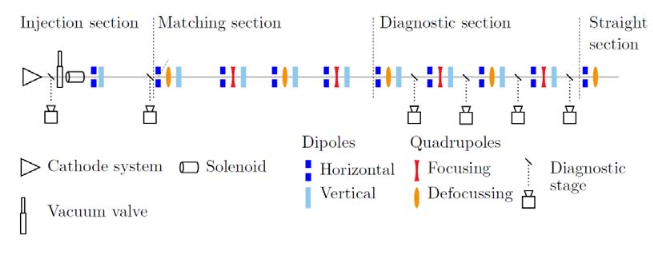
\includegraphics[width=0.8\textwidth]{./salome_aufbau.png}
  \caption{}
\end{figure}
